\section{Students' Background \& Responses}
\label{sec:responses}

In this section we present the background of our students in the technologies
relevant to the course and to the assignment. Then we present the responses
given by the students to our questionnaire. The questions are listed in Tables
\ref{tab:likert} and \ref{tab:comparisons}.

\todo[inline,color=cyan,author=Pedro]{Improve figure colorscheme}

\subsection{Background}

The course of Concurrent, Parallel and Distributed Computing is offered to
students of both the graduate and undergraduate programs in Computer Science at
the University of São Paulo. To gauge the proficiency and knowledge of our
students we elaborated a five-point scale from \textit{Do not Know} $(1)$ to
\textit{Expert or Proficient} $(5)$.  The students were asked to express their
proficiency level on this scale, and their responses are shown in Figure
\ref{fig:background}.

\begin{figure}[htpb]
    \centering
    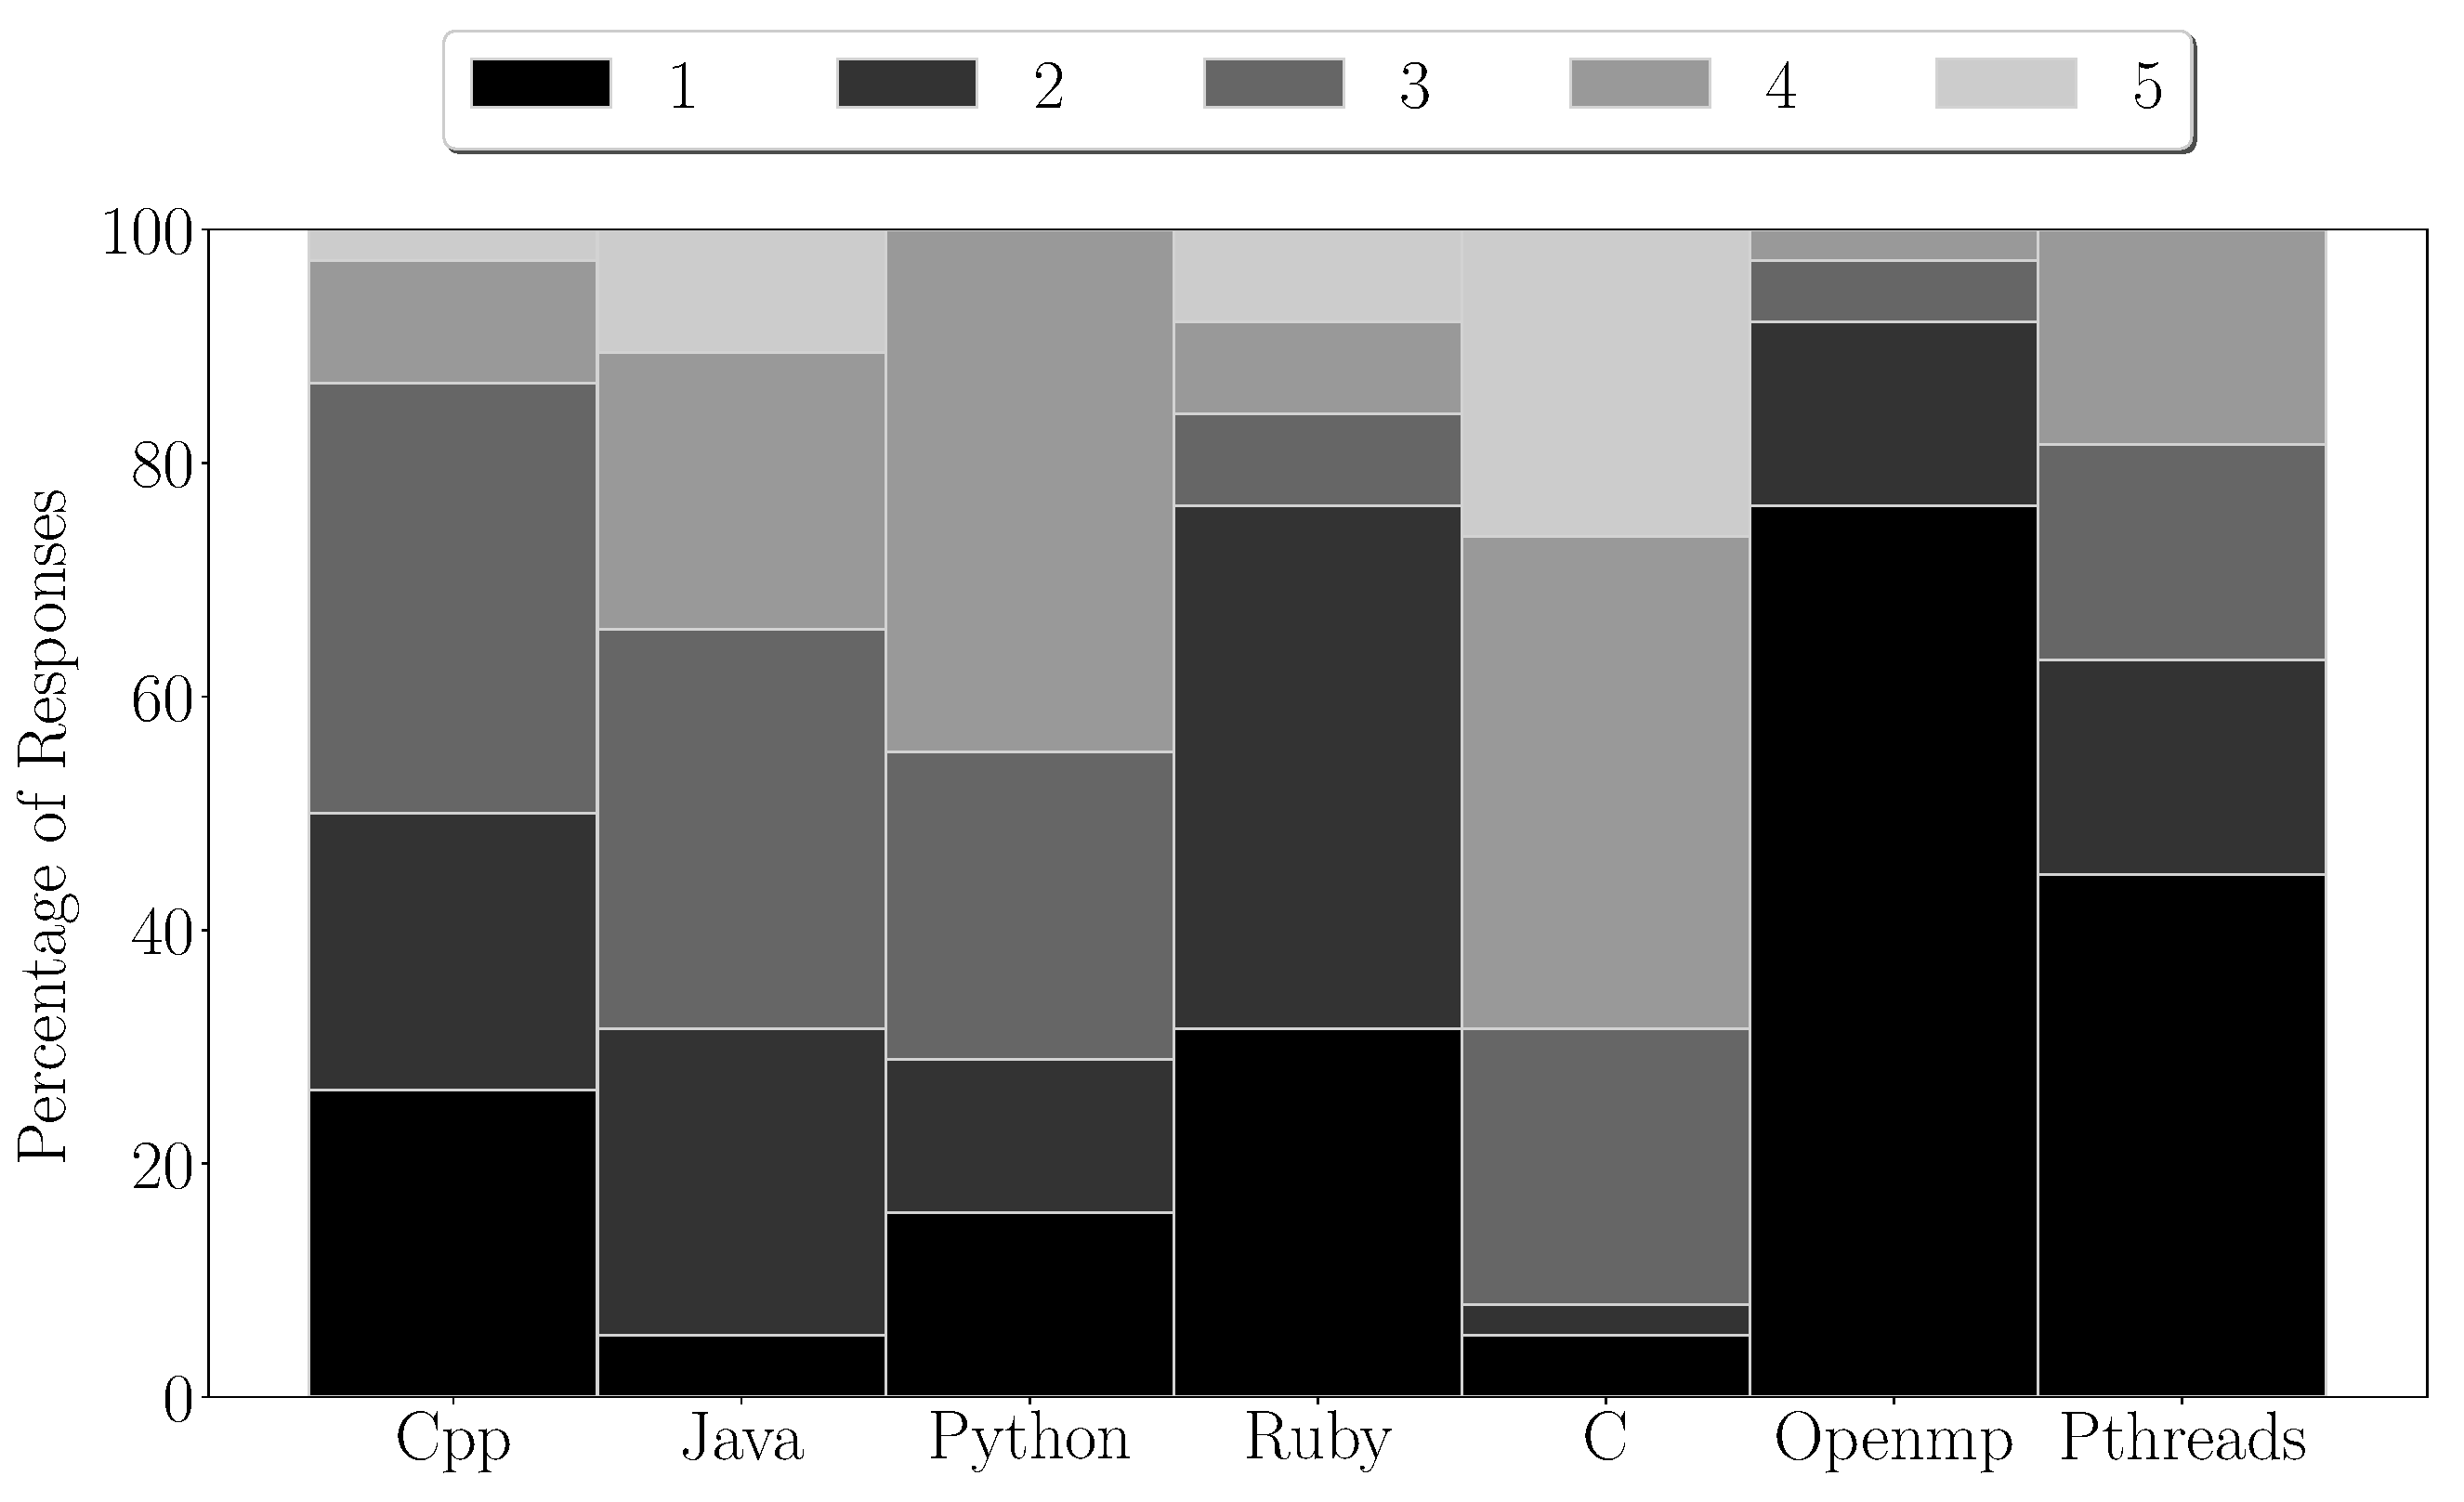
\includegraphics[width=0.85\columnwidth]{background_questions}
    \caption{Student knowledge \textit{before} the assignment}
    \label{fig:background}
\end{figure}

It is common for Computer Science introductory and advanced courses in the
graduate and undergraduate programs of the University of São Paulo to be given
in programming languages such as C, Java and Python. Figure
\ref{fig:background} shows that students reported higher proficiency in those
languages. The C language was the one with which students reported most
proficiency.

The students were asked to evaluate their proficiency in \textit{OpenMP} and
\textit{Pthreads}, \textit{before} completing the assignment, with two sets of
questions. The first set used the same five-point scale as the other background
questions and is also shown in Figure \ref{fig:background}. The students
reported significantly larger proficiency in \textit{Pthreads} than
\textit{OpenMP}, and the majority of the students reported they did not know
\textit{OpenMP} before the course.

\begin{table}[htpb]
    \centering
    \begin{tabular}{@{}p{0.9\columnwidth}p{0.08\columnwidth}@{}}
        \toprule
        \multicolumn{1}{c}{\scriptsize{Have you$\dots$}} & \textnumero \\ \midrule
        \scriptsize{Had contact with parallel and distributed concepts before?} & $(1)$ \\
        \scriptsize{Had contat with the APIs before?} & $(2)$ \\
        \scriptsize{Learned from the OpenMP class?} & $(3)$ \\
        \scriptsize{Learned from the Pthreads class?} & $(4)$ \\ \bottomrule
    \end{tabular}
    \caption{Questions for Figure \ref{fig:classes}}
    \label{tab:classes}
\end{table}

The second set of questions regarding student proficiency with the APIs
comprised the 4 \textit{Yes or No} questions listed in Table \ref{tab:classes}.
This set of questions also asked the students to evaluate whether the classes
on each subject helped their understanding and learning of the technologies.
The student responses for this set are shown in Figure \ref{fig:classes}.  The
majority of the students have had previous contact with the concepts related to
concurrent, parallel and distributed programming, but the majority also have
not had contact or experience with \textit{OpenMP} or \textit{Pthreads}.  Most
students reported that the classes on each API helped their learning.

\begin{figure}[htpb]
    \centering
    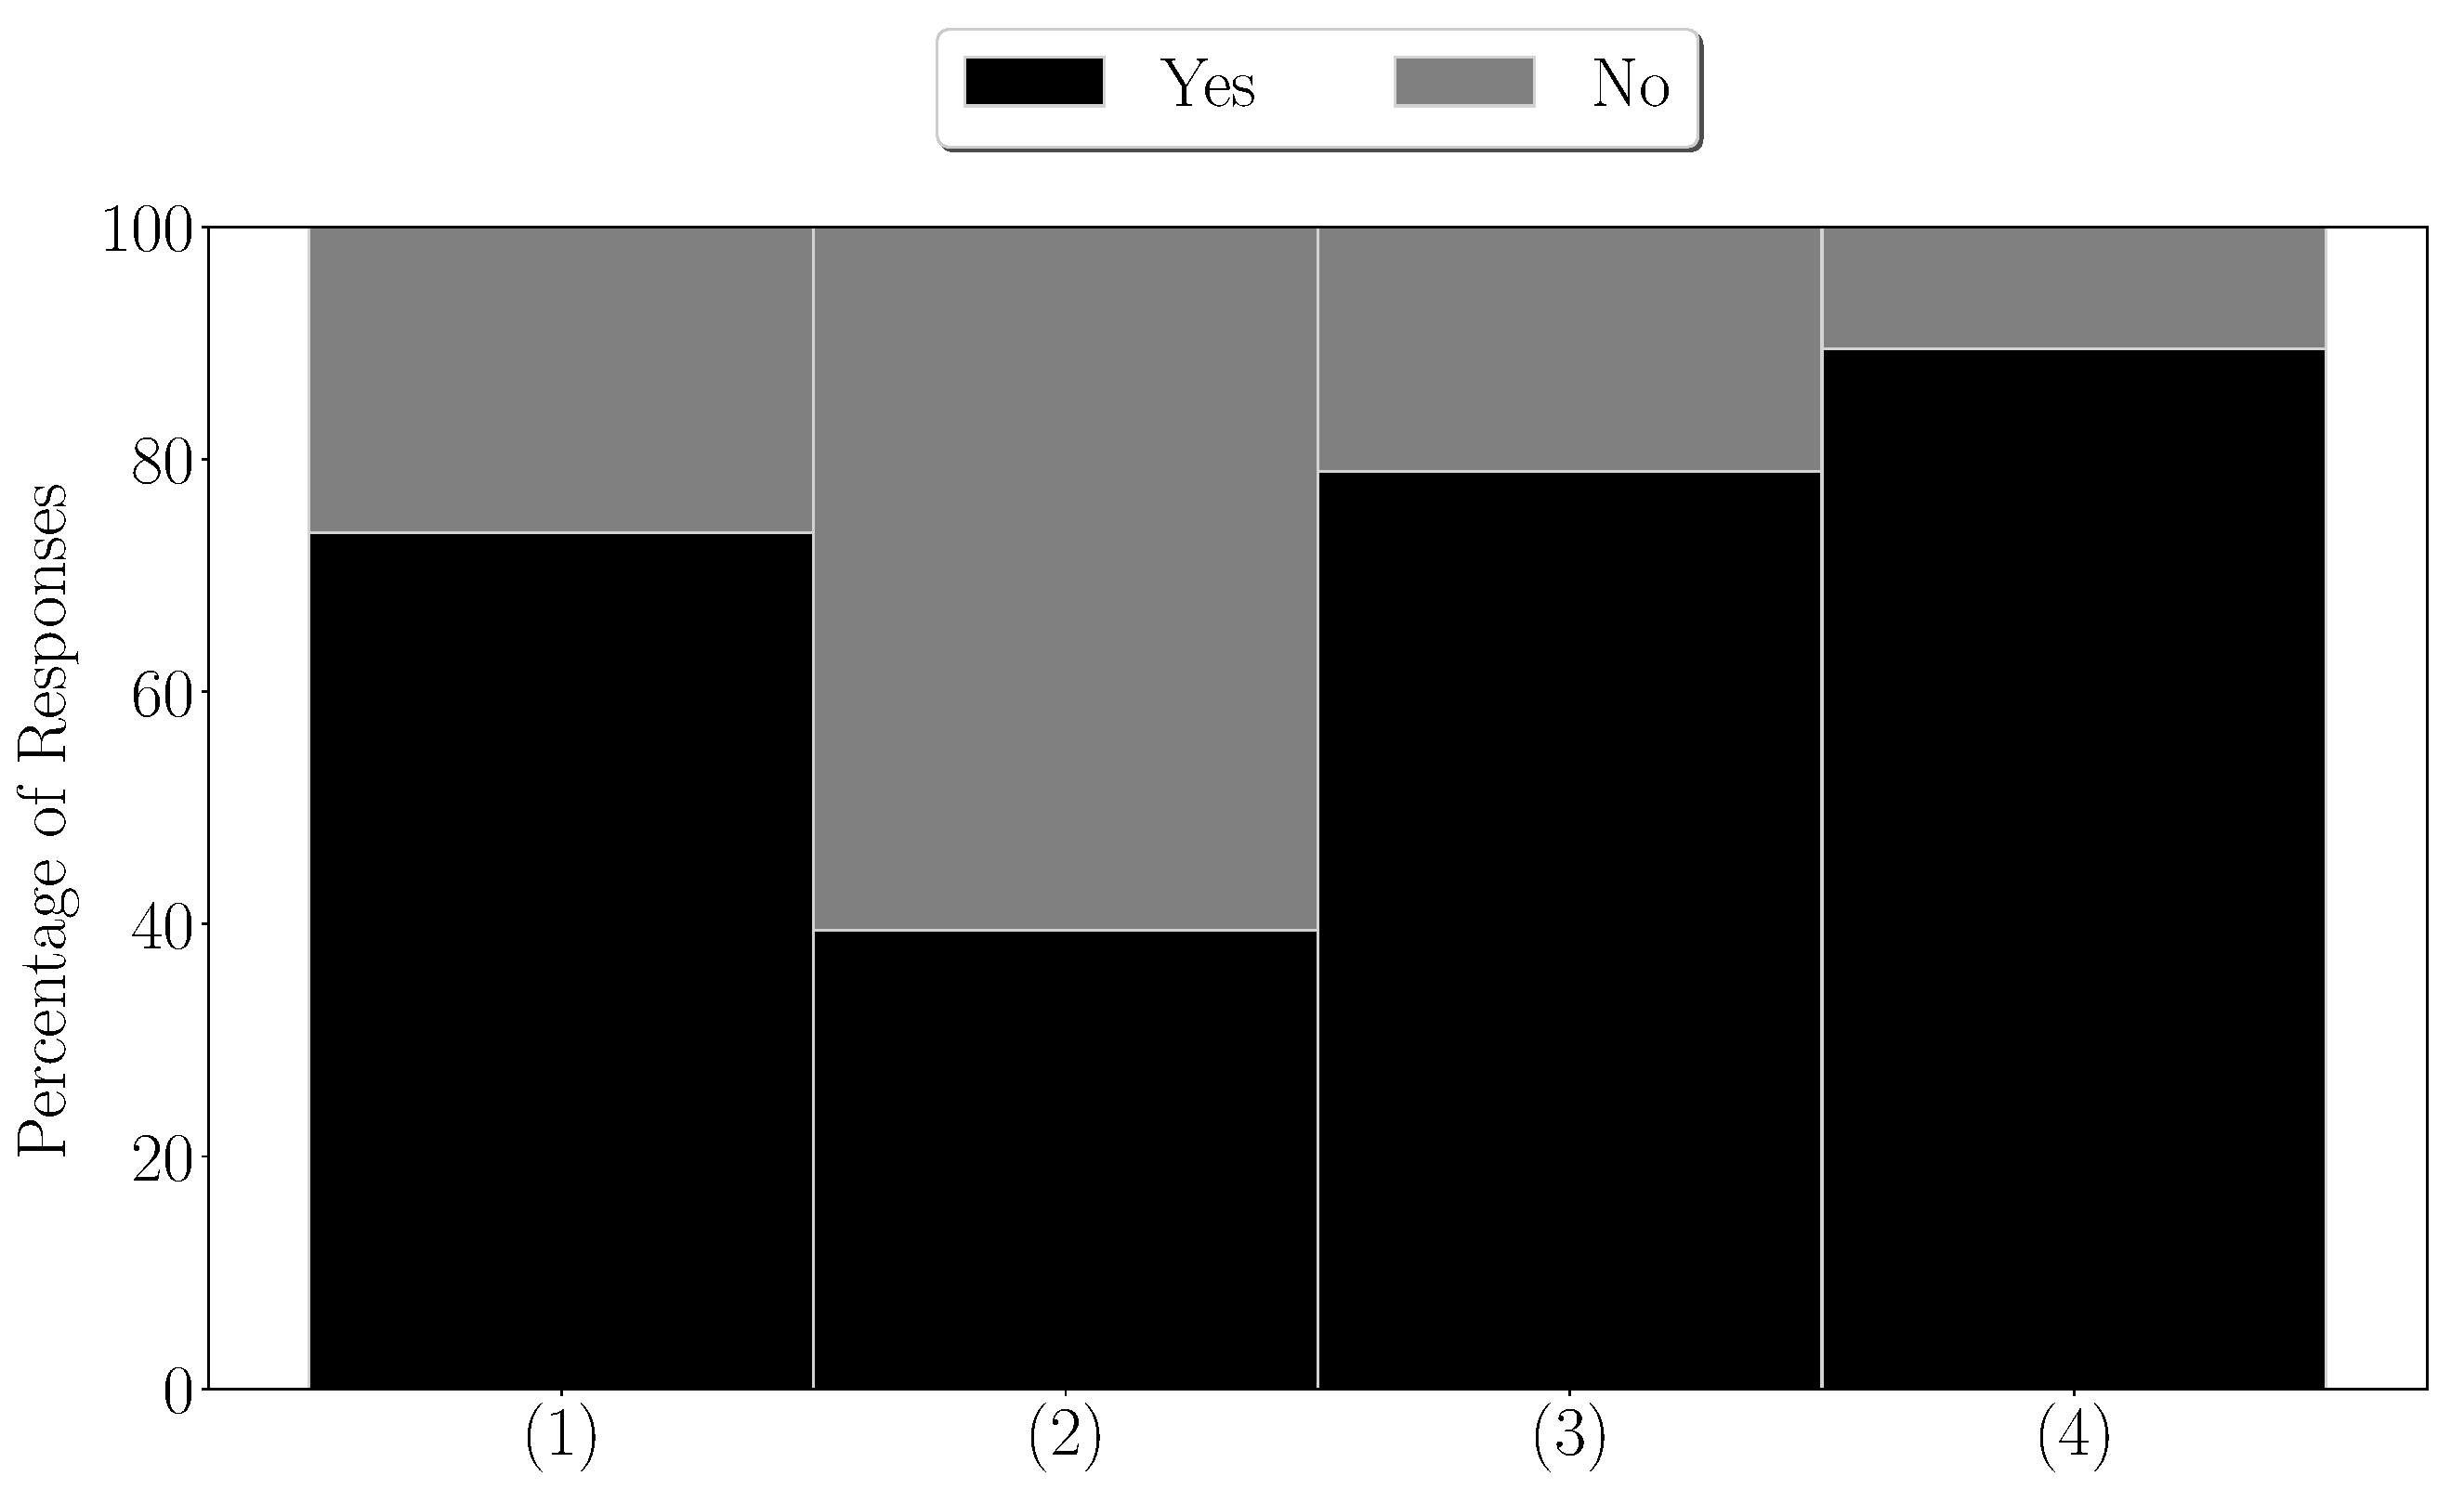
\includegraphics[width=0.85\columnwidth]{classes_questions}
    \caption{Student API knowledge \textit{before} the assignment and their relation to classes}
    \label{fig:classes}
\end{figure}

\subsection{Responses}

The students were asked to answer 3 sets of questions regarding their
experience with \textit{OpenMP} and \textit{Pthreads}, \textit{after}
completing the assignment.
The first set of questions used a Likert-type Scale to measure the relationship
of the students with the two APIs in the context of the assignment. The Likert
Scale~\cite{likert1932technique} enables respondents to express their agreement
or disagreement with specific statements. Respondents choose between five
options: \textit{Strongly Agree} (SA), \textit{Agree} (A), \textit{Neutral}
(N), \textit{Disagree} (D) and \textit{Strongly Disagree}.

The questions of the first set are listed in Table \ref{tab:likert}. The
students expressed their agreement or disagreement with statements related to
the difficulty of parallelizing the first loop with independent iterations,
parallelizing the two nested loops with independent iterations and improving
the performance of the sequential code. Each question was repeated for
\textit{OpenMP} and \textit{Pthreads}, in a total of $6$ questions.

\begin{table}[htpb]
    \centering
    \begin{tabular}{@{}p{0.7\columnwidth}p{0.1\columnwidth}p{0.05\columnwidth}@{}}
        \toprule
        \multicolumn{2}{c}{\scriptsize{It is easy to$\dots$}} & \textnumero \\ \midrule
        \multirow{2}{*}{\parbox{0.7\columnwidth}{\scriptsize{Parallelize loops with independent iterations using:}}} & \scriptsize{OpenMP} & $(1)$ \\
        & \scriptsize{Pthreads} & $(2)$ \\
        \addlinespace{}
        \multirow{2}{*}{\parbox{0.7\columnwidth}{\scriptsize{Parallelize nested loops with independent iterations using:}}} & \scriptsize{OpenMP} & $(3)$ \\
        &  \scriptsize{Pthreads} & $(4)$ \\
        \addlinespace{}
        \multirow{2}{*}{\parbox{0.7\columnwidth}{\scriptsize{Improve the performance of sequential code using:}}} & \scriptsize{OpenMP} & $(5)$  \\
        &  \scriptsize{Pthreads} & $(6)$ \\ \bottomrule
    \end{tabular}
    \caption{Likert-like Scale questions for Figure \ref{fig:likert}}
    \label{tab:likert}
\end{table}

Figure \ref{fig:likert} shows a visualization of the students' responses.  The
height of each stacked sub-column represents the percentage of respondents that
selected each of the correspondent Likert scale agreement levels, which are
represented by different colors.

\begin{figure}[htpb]
    \centering
    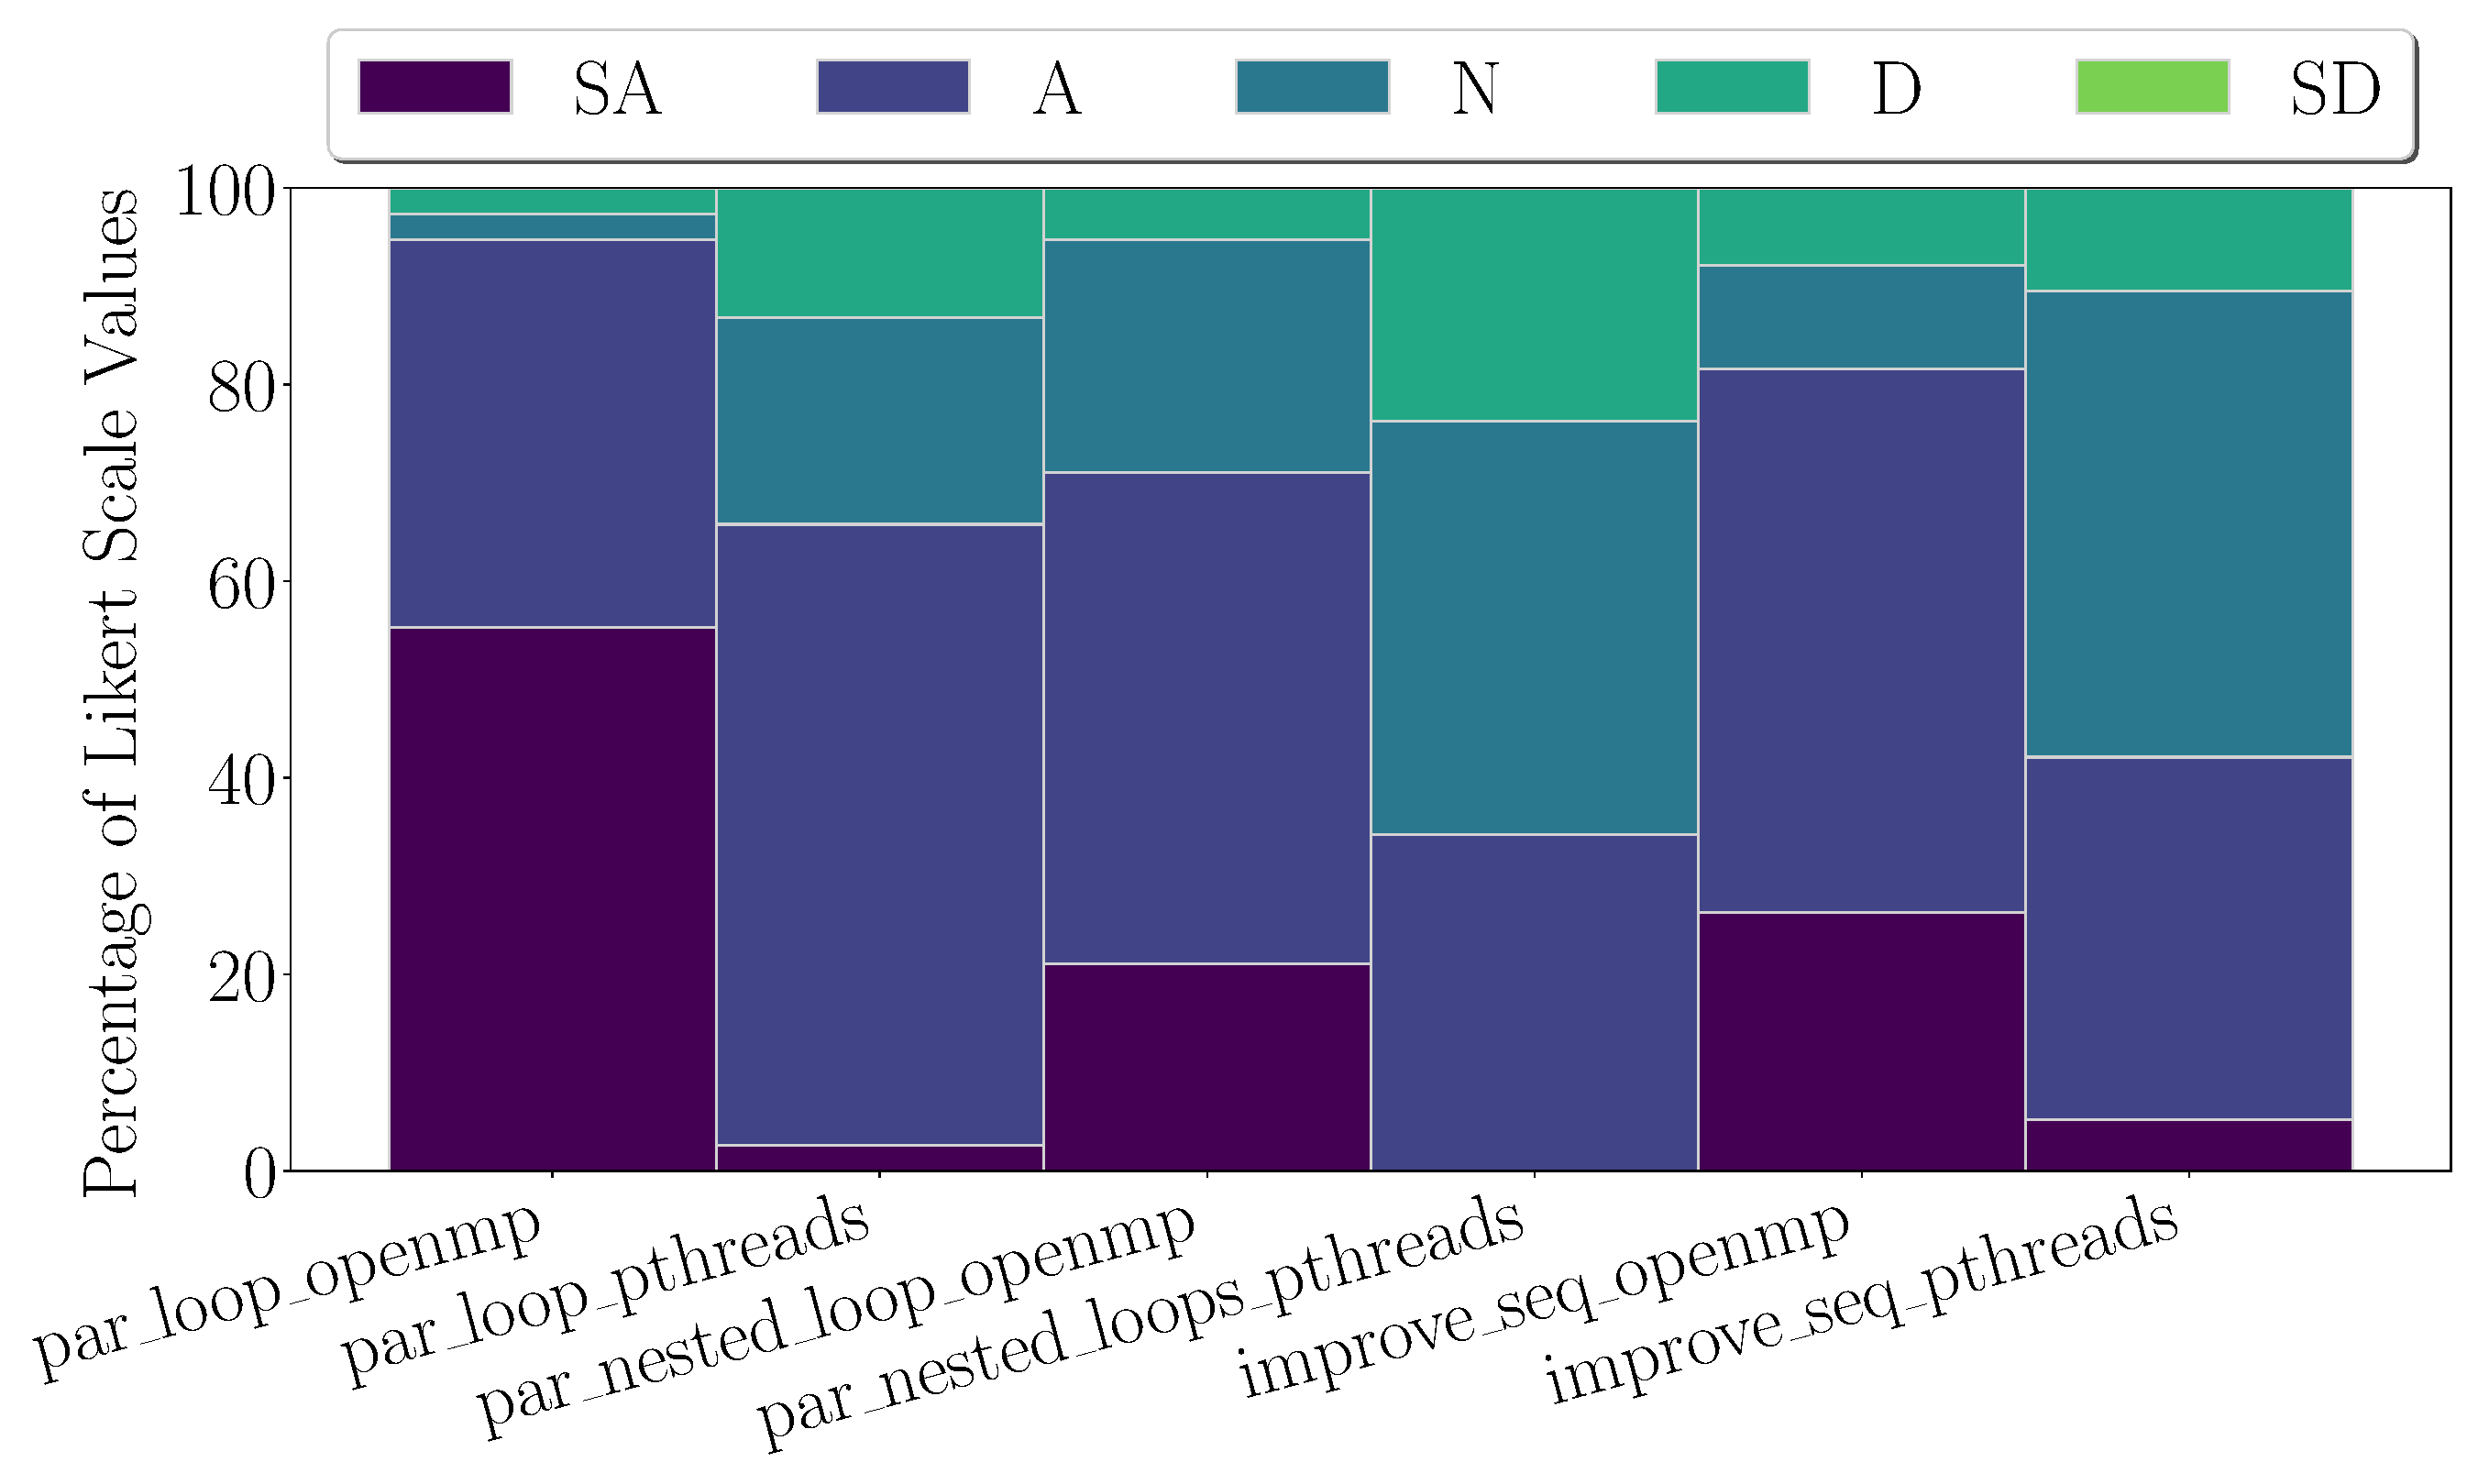
\includegraphics[width=0.85\columnwidth]{likert_questions}
    \caption{Student responses to the Likert Scale questions in Table \ref{tab:likert}}
    \label{fig:likert}
\end{figure}

The percentages of \textit{Strongly Agree} (SA) and \textit{Agree} (A)
responses are significantly larger for questions $(1)$, $(3)$ and $(5)$, which
are related to \textit{OpenMP}.  Likewise, the percentages of \textit{Disagree}
(D) responses are significantly larger for questions $(2)$, $(4)$ and $(6)$,
which are related to \textit{Pthreads}. These responses lead to the conclusion
that \textbf{the perception of the students was that it was easier to use
\textit{OpenMP} than \textit{Pthreads}} to parallelize and improve the
performance of the sequential code provided in the assignment.

The second set of questions used a five-point scale to measure the difficulty
the students had with the learning process of the two APIs for the assignment.
Respondents expressed their difficulty to learn \textit{OpenMP} and
\textit{Pthreads} in a scale of $1$ to $5$, choosing a point between \textit{No
Difficulty} $(1)$ and \textit{Much Difficulty} $(5)$.

Figure \ref{fig:learning} shows a visualization of the students' responses.
The height of each stacked sub-column represents the percentage of respondents
that selected each of the correspondent difficulty levels, which are
represented by different colors.

\begin{figure}[htpb]
    \centering
    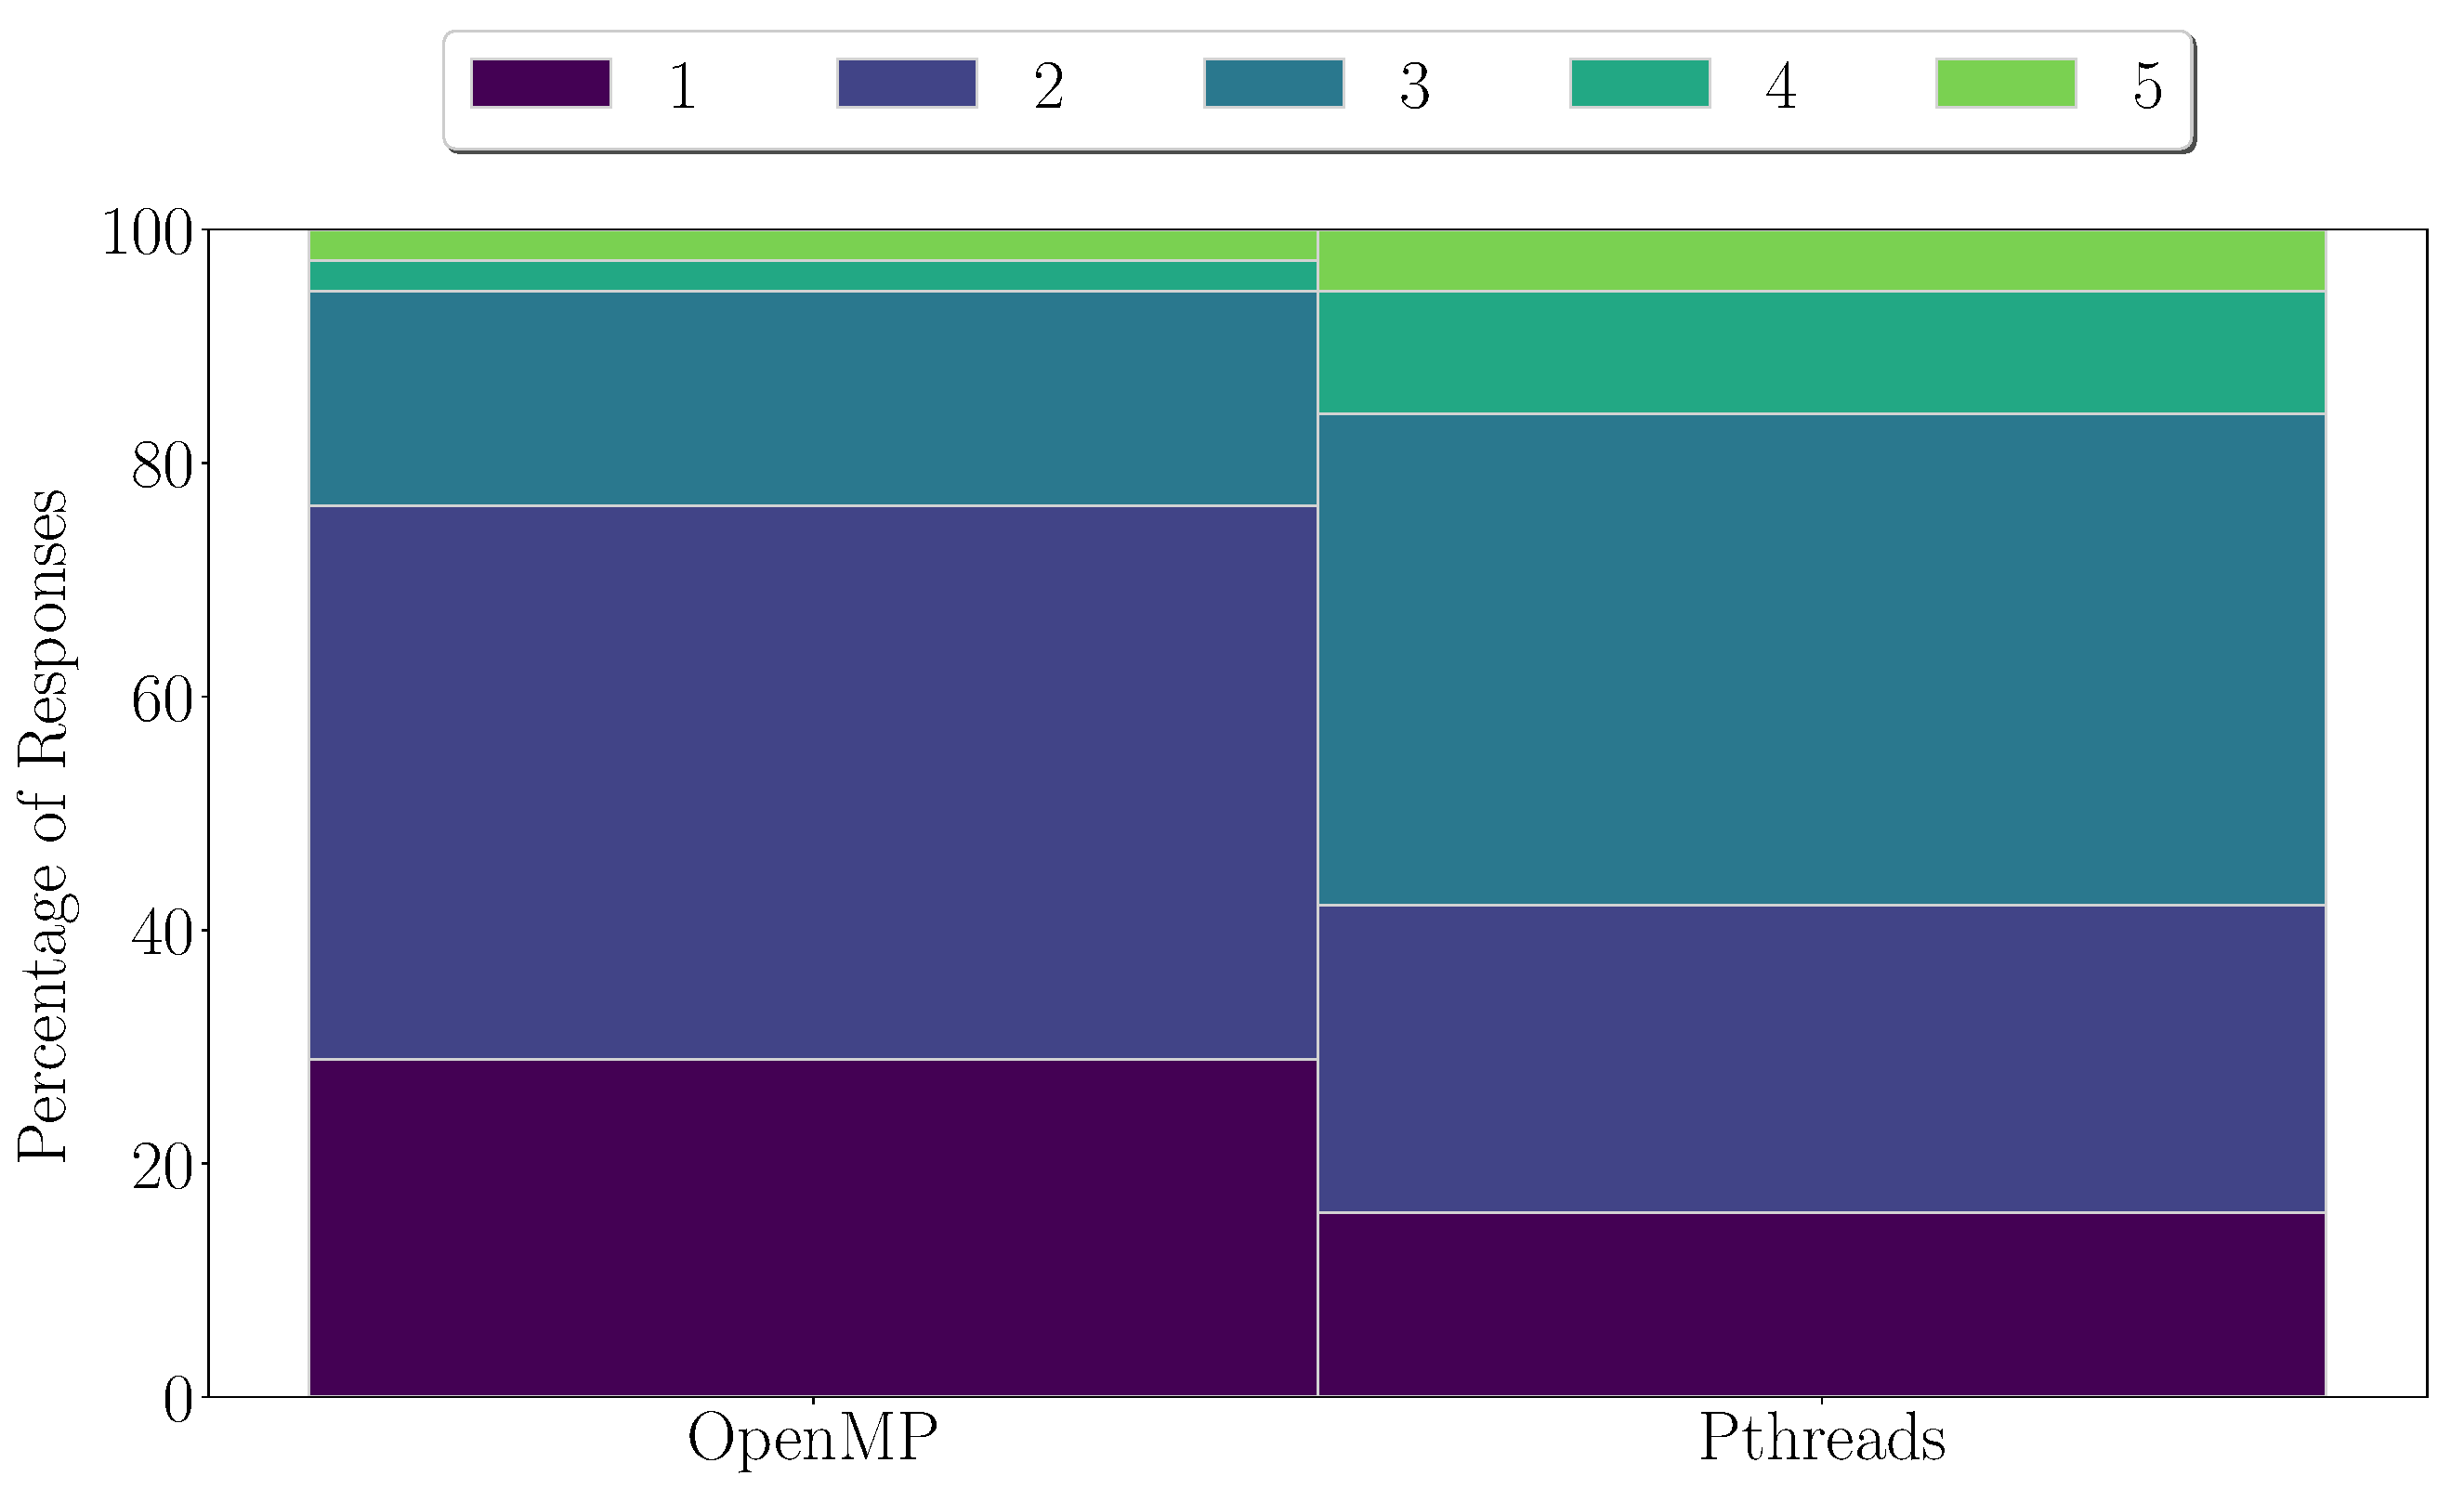
\includegraphics[width=0.85\columnwidth]{learning_difficulty_questions}
    \caption{Student difficulty to learn the APIs in a five-point scale}
    \label{fig:learning}
\end{figure}

The percentages of \textit{No Difficulty} $(1)$ and difficulty level $(2)$
responses are significantly larger for learning \textit{OpenMP}. Likewise, the
percentages of difficulty level $(4)$ and \textit{Much Difficulty} $(5)$
responses are significantly larger for learning \textit{Pthreads}.  We derive
from these responses the conclusion that \textbf{the students perceived less
difficulty to learn \textit{OpenMP} than \textit{Pthreads}} for the purposes of
the assignment.

The final set of questions regarding the usage and learning of \textit{OpenMP}
and \textit{Pthreads} in the context of the first assignment presented
comparison questions between the two APIs. Students chose which API they
perceived was the best answer to the questions in Table \ref{tab:comparisons}.

Responses to question $(13)$ in Table \ref{tab:comparisons} were not obtained
directly from the students. We analysed each assignment submission and
evaluated the performance of the each solution across the specified
experimental settings.

\begin{table}[htpb]
    \centering
    \begin{tabular}{@{}p{0.9\columnwidth}p{0.08\columnwidth}@{}}
        \toprule
        \multicolumn{1}{c}{\scriptsize{Which technology$\dots$}} & \textnumero \\ \midrule
        \scriptsize{Was more difficult to learn?} & $(7)$ \\
        \scriptsize{Was simpler to use?} & $(8)$ \\
        \scriptsize{Was easier to use?} & $(9)$ \\
        \scriptsize{Was easier to use for parallelizing loops with independent iterations?} & $(10)$ \\
        \scriptsize{Was easier to use for parallelizing nested loops with independent iterations?} & $(11)$  \\
        \scriptsize{Was easier to use for improving the performance of a sequential program?} & $(12)$  \\
        \scriptsize{Had the best performance on your assignment?} & $(13)$ \\ \bottomrule
    \end{tabular}
    \caption{Questions for Figure \ref{fig:comparisons}}
    \label{tab:comparisons}
\end{table}

Figure \ref{fig:comparisons} shows a visualization of the students' responses.
The height of each stacked sub-column represents the percentage of respondents
that selected each API, which are represented by different colors.

The percentage of \textit{OpenMP} selections is significantly larger for all
questions, except for questions $(7)$ and $(13)$. The responses for questions
$(7)$ -- $(12)$ strengthen the previous conclusion that the perception of the
students was that it was easier to use \textit{OpenMP} than \textit{Pthreads}
in the context of the assignment. The performance results that we obtained from
analysing the students' submissions challenge the perception of the students.
The responses to question $(13)$, extracted by our analysis, show that
\textbf{the students achieved better performance when using \textit{Pthreads}
than \textit{OpenMP}}.

\begin{figure}[htpb]
    \centering
    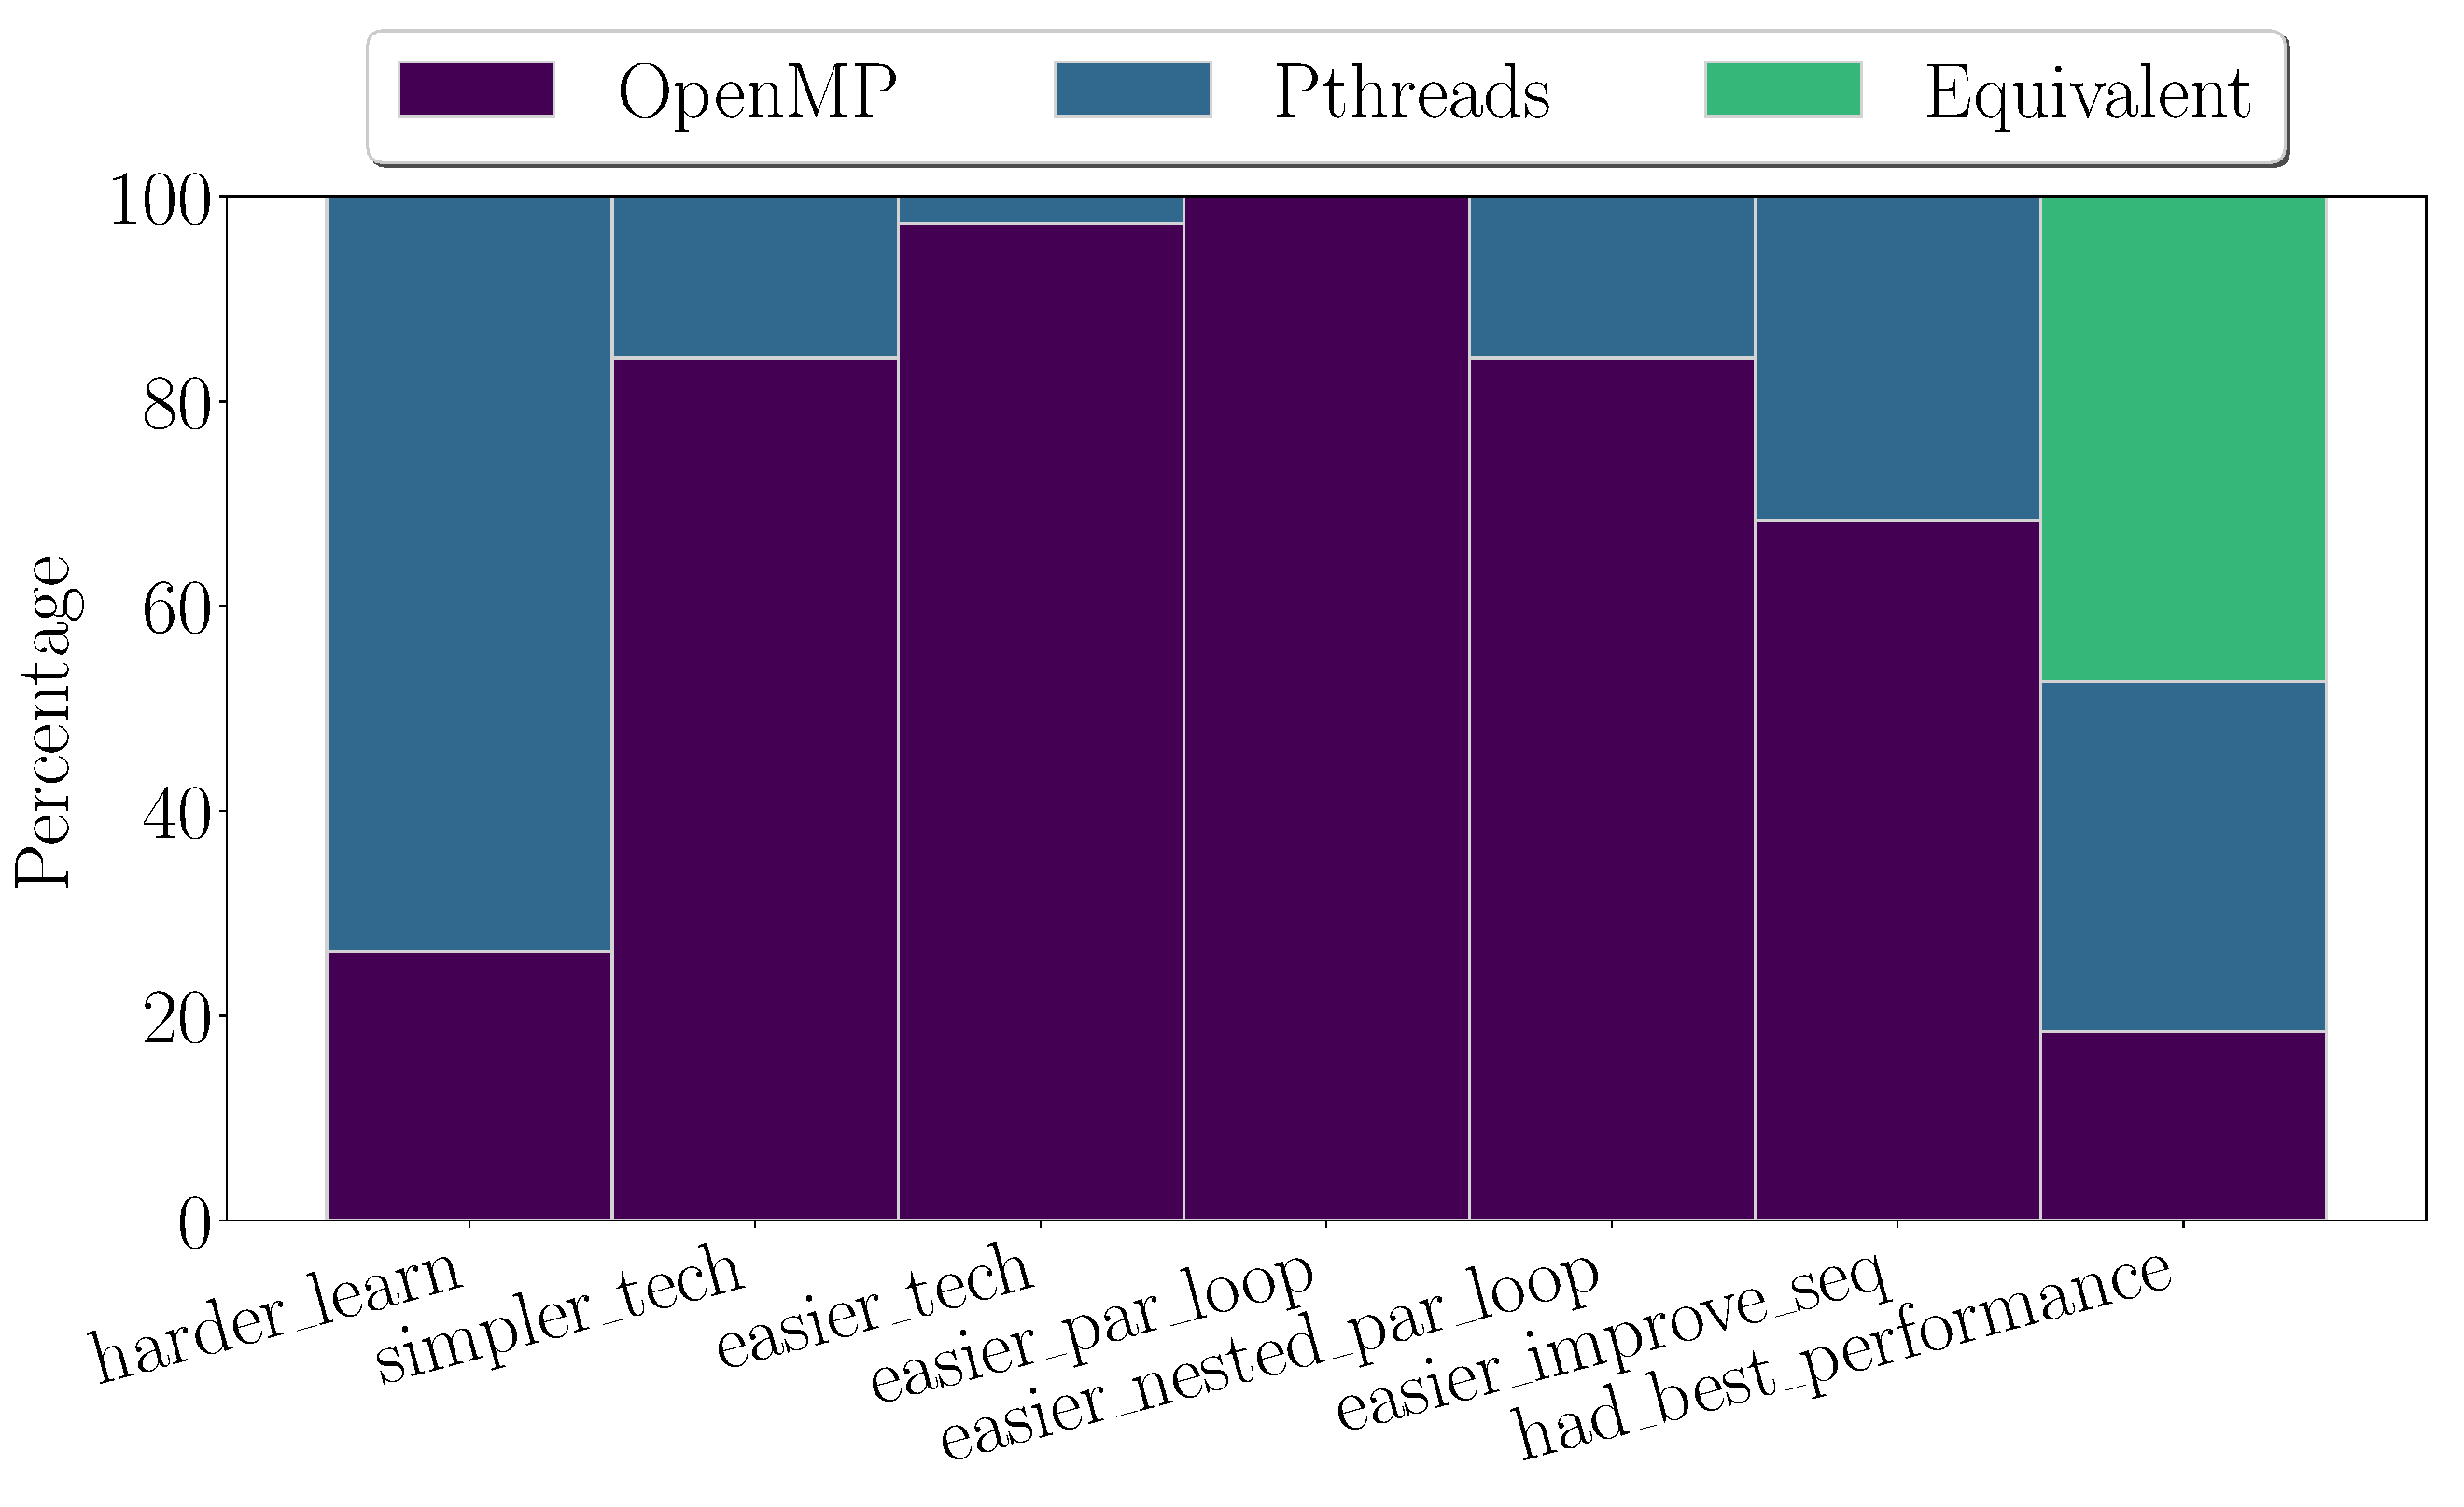
\includegraphics[width=0.85\columnwidth]{comparisons}
    \caption{Student responses to the questions in Table \ref{tab:comparisons}}
    \label{fig:comparisons}
\end{figure}

\todo[inline,color=cyan,author=Pedro]{Improve these last paragraphs}

The responses presented in this section enable the conclusion that the students
perceived less difficulty using and learning \textit{OpenMP} in the context
of the assignment. They also reported the perception that using \textit{OpenMP}
made it easier to improve the performance of the sequential code we provided.
Our analysis of the submissions revealed that the majority of the students
($52.2\%$) achieved better performance in the assignment with either
\textit{OpenMP} ($17.4\%$) or \textit{Pthreads} ($34.8\%$). Contradicting the
perception of the students, the implementation using \textit{Pthreads} achieved
better performance in twice the submissions.

This shows that the perceptions of usability and performance improvement
regarding \textit{OpenMP} did not reflect in the actual implementations and
submissions. We believe that \textit{OpenMP} is still not as easy as it appears
to be, and that the students' responses strengthen the argument for teaching
lower-level technologies for parallel and distributed computing.
